\section{问题三：多因素约束下的NIPT时点优化决策}
问题三的目标是综合孕妇的身高、体重、年龄与身体质量指数BMI等多种因素，在满足特定Y染色体浓度达标比例的前提下，为通过BMI划分的不同孕妇群体制定风险最小化的最优NIPT检测时点。为达成此目标，本文构建了一个职责分离的建模框架。该框架首先利用全体样本数据进行客观的孕妇分群，随后在提纯后的高质量数据子集上训练一个包含多因素的稳健预测模型，最终将分群与预测结果结合，通过带约束的多目标优化方法求解各群组的最优检测策略。具体流程如图\ref{fig:q3_framework}所示。

\begin{figure}[h!]
    \centering
    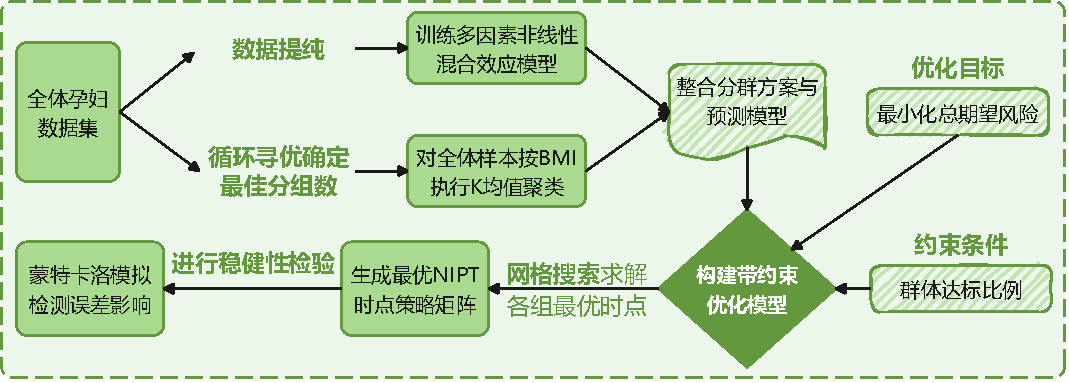
\includegraphics[width=\textwidth]{figs/5问题三/问题三.pdf}
    \caption{问题三的建模框架}
    \label{fig:q3_framework}
\end{figure}

\subsection{基于全体样本的孕妇分群}
为保证分组的普适性，分群过程在包含全部998条记录的完整数据集上进行。依据题目的要求，我们仅使用孕妇BMI这单一维度特征作为分组依据。本文选择K均值聚类算法对全体孕妇进行分组。

最优分组数量K的选择，是基于最终优化目标的反馈来决定的。本文遍历不同的分组数量K，从2至8。对每一种K值下的分组方案，都执行后续的完整优化流程，计算出该方案对应的全体孕妇的加权平均总风险。最终选择使该全局风险指标最小的K值，作为最优的分组数量。

\begin{figure}[H]
    \centering
    \begin{minipage}[t]{0.48\textwidth}
        \centering
        
\includegraphics[width=\textwidth]{figs/5问题三/图_第三问_最优K值决策图.png}
        \caption{基于总风险最小化的最优分组数决策}
        \label{fig:q3_k_decision}
    \end{minipage}
    \hfill
    \begin{minipage}[t]{0.48\textwidth}
        \centering
        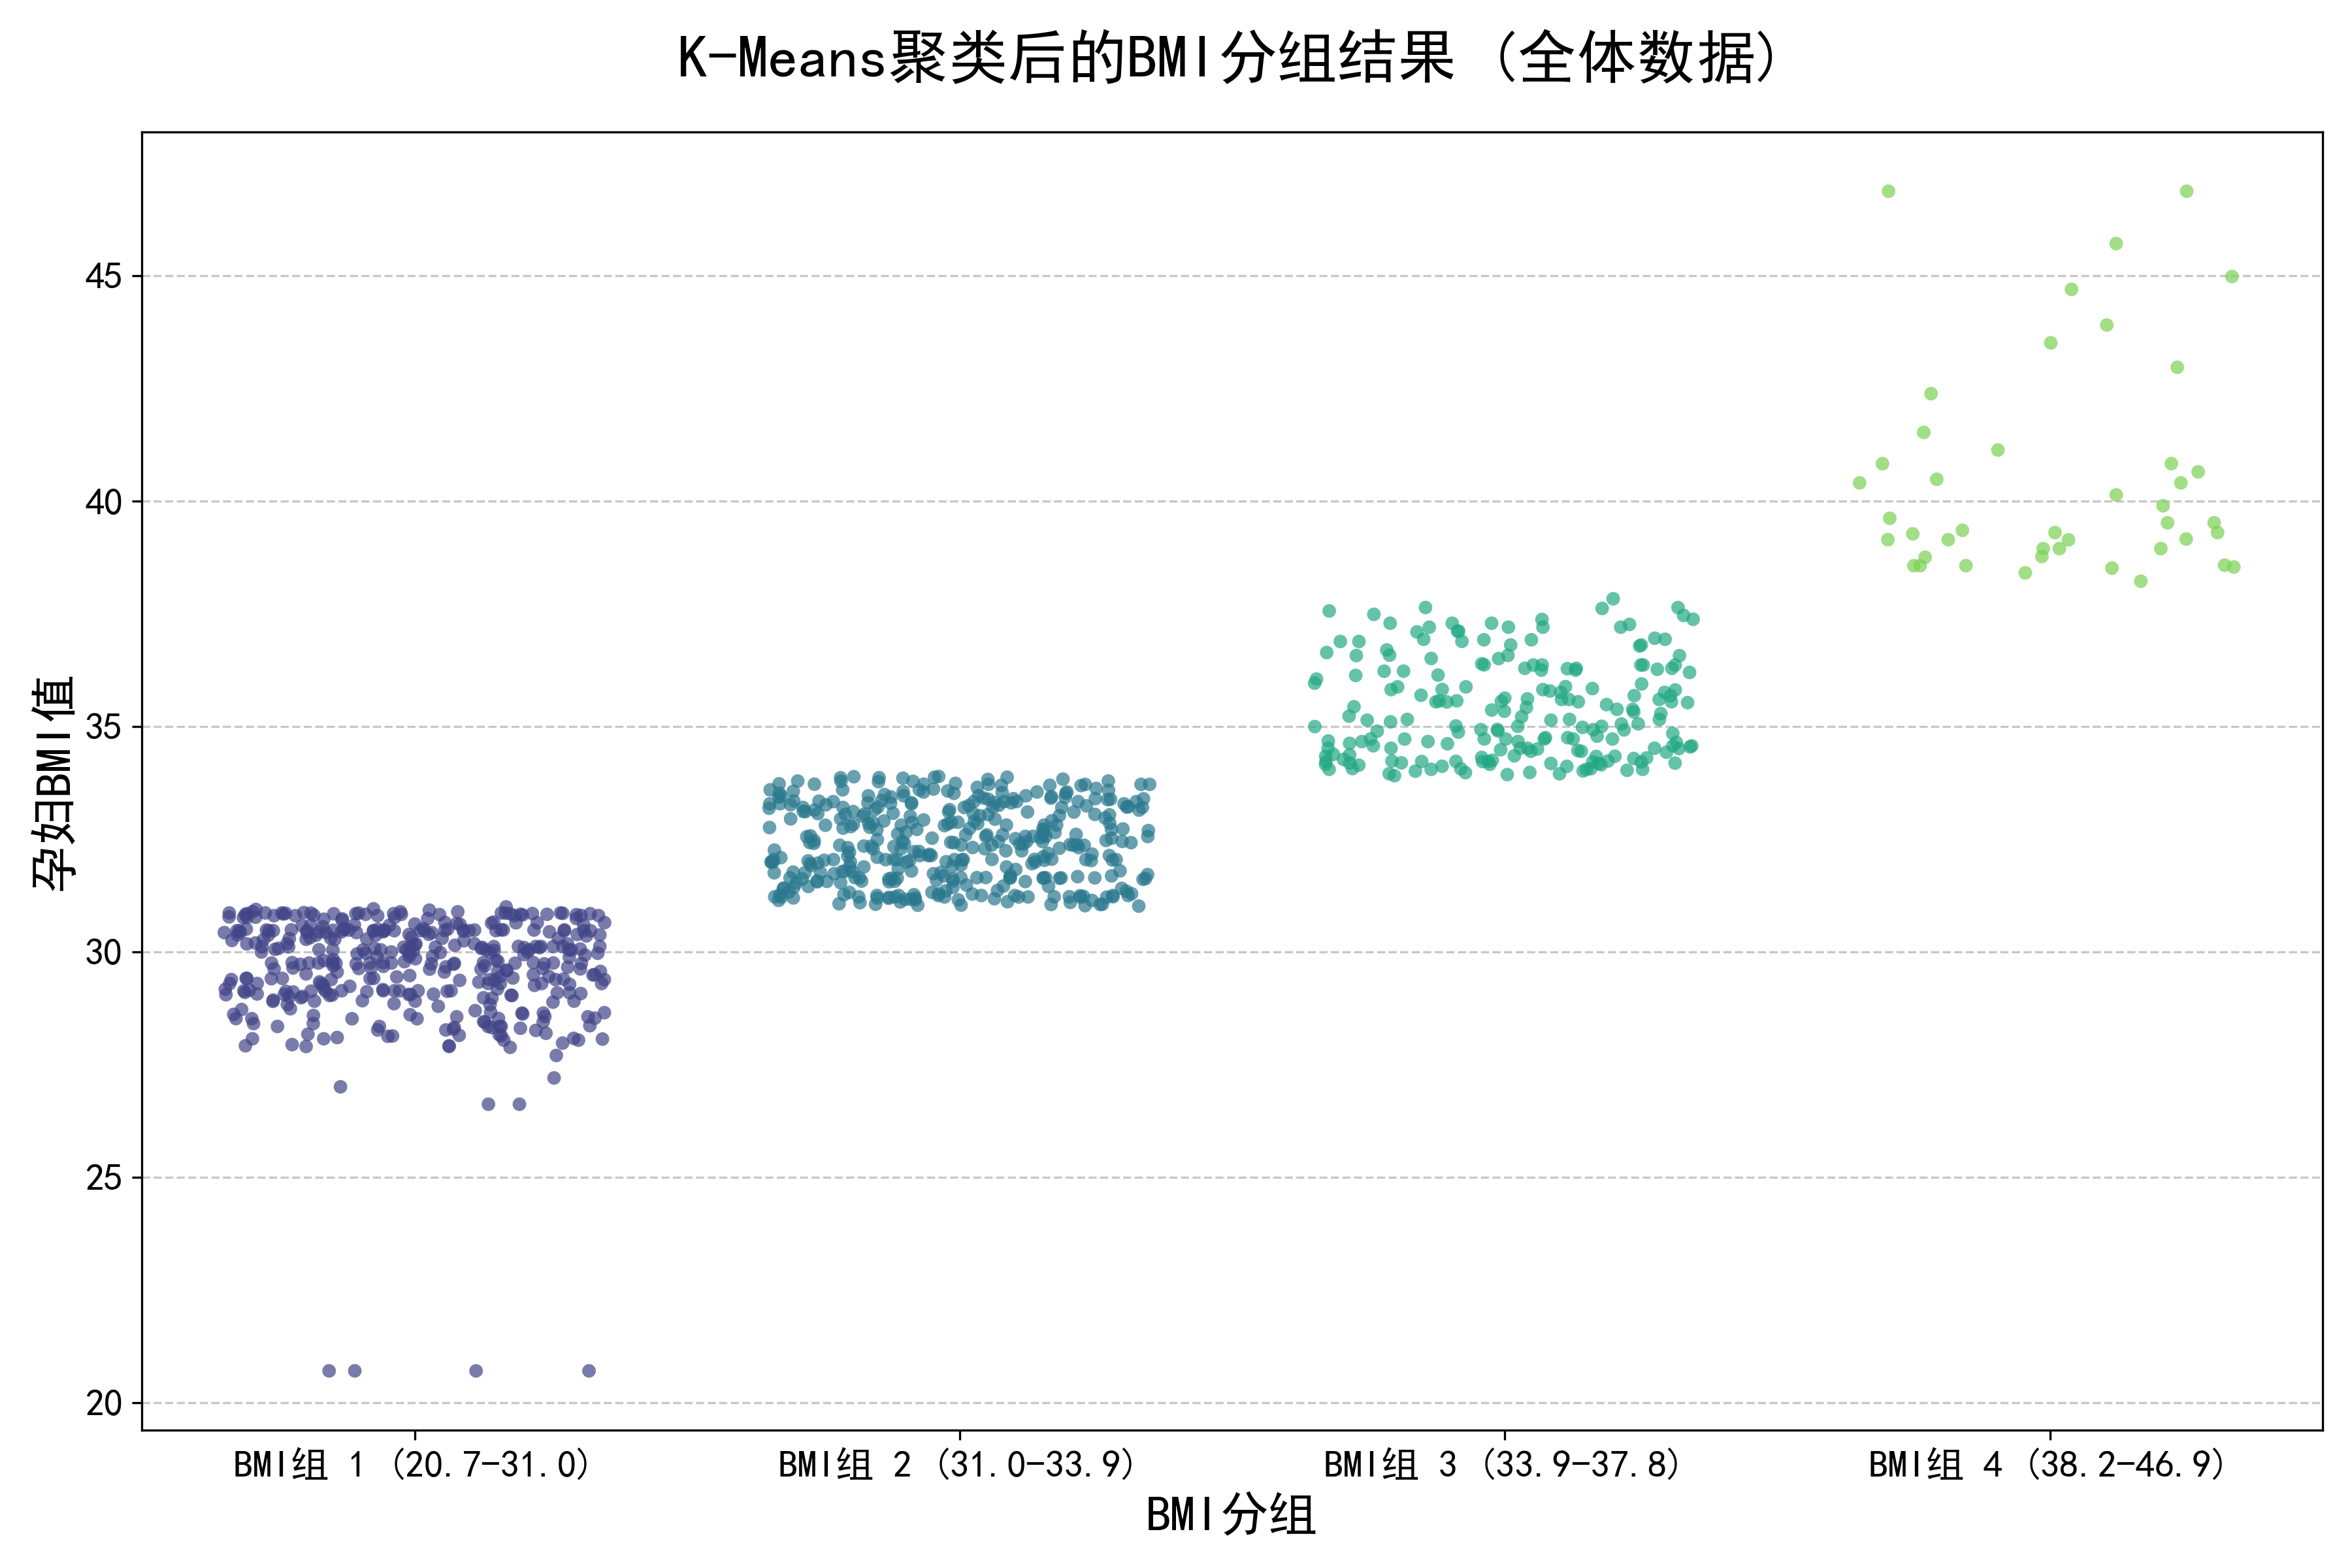
\includegraphics[width=\textwidth]{figs/5问题三/图_第三问_KMeans聚类结果.png}
        \caption{最优分组数K等于4时的BMI聚类结果}
        \label{fig:q3_kmeans_results}
    \end{minipage}
\end{figure}

\cref{tab:model_performance}对各模型在测试集上的性能指标进行了量化总结。数据显示，决策树模型虽然获得了最高的异常类召回率0.6316，但其精确率仅为0.2034，是三者中最低的，这表明该模型倾向于将大量正常样本误判为异常。相比之下，逻辑回归模型在各项指标上表现出更优的综合性能：其异常类F1分数0.4390和AUC值0.8045均为最高，这意味着它在精确率和召回率之间取得了最优的平衡，且整体判别能力最强。尽管XGBoost的精确率略高于逻辑回归，但其召回率过低，导致F1分数不理想。综合考量，逻辑回归模型因其平衡性和整体性能，被选定为最终的判定模型。


不同K值对应的加权平均总风险计算结果展示于\cref{fig:q3_k_decision}。图中横坐标为聚类数量K，纵坐标为加权平均总风险。曲线显示，当分组数K等于4时，总风险达到所有候选方案中的最低点。因此，本文最终确定K等于4为最优分组数。



依据最优分组数4，K均值聚类算法在全体样本上的划分结果如\cref{fig:q3_kmeans_results}所示。该图展示了四个沿身体质量指数分布的孕妇群组。最终确定的四个群组及其身体质量指数范围分别为：组1，范围20.7至31.0；组2，范围31.0至33.9；组3，范围33.9至37.8；组4，范围38.2至46.9。

\subsection{多因素非线性关系预测模型}
为建立一个能预测Y染色体浓度的模型，并减弱离群点对模型参数估计的干扰，本阶段先进行数据处理。从完整的998条记录出发，对孕周，身高，体重，年龄，孕妇身体质量指数与Y染色体浓度六个核心变量，逐一应用1.5倍四分位距准则进行离群点检测。该过程形成了一个包含931条观测记录的数据集，用于后续预测模型的训练。

模型类型上，本文选择非线性混合效应模型，以捕捉变量间的非线性关系以及孕妇间的个体差异。同时，为模拟真实检测中存在的随机波动，模型中加入了代表检测误差的高斯噪声项。根据在处理后数据集上的拟合结果，最终确立的预测模型表达式为：
\begin{equation}
\begin{aligned}
\hat{Y}_{ij} = u_{0,i} & - 7.1472 \\
& + 4.5615 \times 10^{-3} \cdot \text{孕天数}_{ij} - 3.4421 \times 10^{-5} \cdot \text{孕天数}_{ij}^2 + 9.5710 \times 10^{-8} \cdot \text{孕天数}_{ij}^3 \\
& + 0.1274 \cdot \text{BMI}_{ij} - 9.7171 \times 10^{-4} \cdot \text{BMI}_{ij}^2 \\
& + 5.9349 \times 10^{-3} \cdot \text{年龄}_{ij} - 8.5600 \times 10^{-5} \cdot \text{年龄}_{ij}^2 \\
& - 0.0449 \cdot \text{体重}_{ij} + 1.1372 \times 10^{-4} \cdot \text{体重}_{ij}^2 \\
& + 0.0581 \cdot \text{身高}_{ij} - 9.8937 \times 10^{-5} \cdot \text{身高}_{ij}^2 \\
& + 9.1773 \times 10^{-6} \cdot (\text{孕天数}_{ij} \times \text{孕妇BMI}_{ij}) \\
& - 1.6636 \times 10^{-5} \cdot (\text{孕天数}_{ij} \times \text{年龄}_{ij}) \\
& + \epsilon
\end{aligned}
\end{equation}
其中，$u_{0,i}$是第i位孕妇的随机效应截距，代表了个体特异性，其服从均值为0，方差为$6.965 \times 10^{-4}$的正态分布，即 $u_{0,i} \sim \mathcal{N}(0, 6.965 \times 10^{-4})$。$\epsilon$代表检测误差，服从均值为0的正态分布，$\epsilon \sim \mathcal{N}(0, \sigma^2_{error})$。

\subsection{带约束的时点优化与稳健性检验}
本阶段将分组结果与预测模型整合，以求解各组的最优检测时点。优化模型的目标函数为最小化总期望风险$R_{total}(t_g)$。模型中的关键指标推导如下。基于非线性混合效应模型的预测值$\hat{Y}_i(t)$与残差标准差$\hat{\sigma}_{residual}$，可计算任一孕妇在时间点t的个体达标概率：
\begin{equation}
P_{\text{pass, i}}(t) = 1 - \Phi\left(\frac{0.04 - \hat{Y}_i(t)}{\hat{\sigma}_{residual}}\right)
\end{equation}
一个群组g的群体期望达标比例，定义为该组内所有个体达标概率的算术平均值：
\begin{equation}
P_{\text{rate}}(t_g) = \frac{1}{|I_g|} \sum_{i \in \text{group}_g} P_{\text{pass, i}}(t)
\end{equation}
总期望风险$R_{total}(t)$则由延迟检测的健康风险$R_{late}(t)$与检测失败的机会成本风险$R_{fail}(t)$两部分构成：
\begin{equation}
R_{\text{total}}(t) = R_{late}(t) + R_{fail}(t)
\end{equation}
求解过程采用网格搜索算法，在70天至196天的时间范围内，为每个群组寻找最优时点。


为检验模型结论在面对现实检测误差时的稳健性，本文进行了敏感性分析。通过蒙特卡洛模拟，在非线性混合效应模型的预测值上，叠加一个服从均值为0，标准差为$\sigma_{error}$的正态分布随机误差。

\begin{figure}[H]
    \centering
    
\includegraphics[width=0.8\textwidth]{figs/5问题三/图_第三问_检测误差敏感性分析.png}
    \caption{最优时点对检测误差的敏感性分析}
    \label{fig:q3_sensitivity}
\end{figure}

\cref{fig:q3_sensitivity}中的箱线图展示了BMI最高的组4，在期望达标比例为92.5\%的约束下，随着检测误差标准差$\sigma_{error}$从0.0增大到0.015，最优时点分布的变化。结果显示，随着检测误差的增大，推荐的最优时点均值保持稳定，但分布的离散程度显著增加。这表明本决策框架具有良好的稳健性，即使存在一定的检测误差，推荐的最佳时点均值也不会发生剧烈偏移，保证了决策建议的可靠性。